\chapter{Interferometric stabilisation of reservoir cavity}

\label{ch-stabilisation}

%%%%%%%%%% INTRODUCTION %%%%%%%%%%

\section{Introduction}

In this introductory section, the concept of interferometry is presented. As the name of the chapter suggests, this technique is used to stabilise the reservoir cavity. The reason why an optical cavity needs stabilisation will appear clearer later, but basically, this is due to the fact that light is a wave and that it can interfere with itself inside the cavity. The interferences can be constructive, destructive, or can behave in any intermediate way. Moreover, it will be shown that the interferometric properties are wavelength dependent. Since several wavelengths coexist inside the reservoir, this gives a first glimpse on the complexity entailing its stabilisation. To gain some insight on interferometry, and before moving on to the study of an actual ring cavity, the features of the well known \gls{fp} interferometer are recalled. After that, it is shown that the properties studied for the \gls{fp} can be translated to ring cavities with close to no modification. Finally, under the light of the basic notions of interferometry developed, the difficulties linked to the stabilisation of the reservoir cavity, which is at the heart of the scheme introduced in this thesis, are presented.

%%% FABRY-PEROT INTERFEROMETER %%%

\subsection{Fabry-Perot interferometer}

The \gls{fp} plays an important role in modern optics as it is really ubiquitous. This can be explained by the fact that, despite its great simplicity, it can reach good performance using high reflectivity mirrors, which can be produced using nowadays technologies. In practice, a \gls{fp} cavity is simply made of two facing mirrors as can be viewed on figure \ref{fp}. On this figure, one can see the two mirrors, represented by the vertical black lines, and the different electric fields. The resonance condition, namely the regime where the transmitted electric field $E_{\text{t}}$ is maximum, can be seen intuitively as a situation where the intra-cavity field $E_1$ is in phase with the incident field $E_{\text{in}}$, which leads to the build up of a very intense intra-cavity electric field. On the other hand, the anti-resonance condition is met when $E_{\text{in}}$ and $E_1$ are out of phase. The transmissivity of the \gls{fp} interferometer, which is defined as the ratio $|E_{\text{t}}|^2/|E_{\text{in}}|^2$, is given by \cite{Perot1899}:

\begin{equation}
	\mathcal{T}(\omega) = \frac{1}{1+\mathcal{F}\sin^2{\left(\frac{\omega}{\text{FSR}}\right)}}
	\label{transmissivity}
\end{equation}

In this expression, $\mathcal{F}$ is the finesse of the cavity, $\omega$ is the angular frequency of the incident electric field, and FSR is the \acrlong{fsr} of the cavity. In a stationary regime, the energy inside the cavity does not evolve, therefore the energy carried by the incident electric field $E_{\text{in}}$ can either be transmitted or reflected, which implies that the reflectivity of the cavity which is defined as the ratio $|E_{\text{ref}}|^2/|E_{\text{in}}|^2$ is simply given by:

\begin{equation}
	\mathcal{R}(\omega) = 1 - \mathcal{T}(\omega)
	\label{reflectivity}
\end{equation}

\begin{figure}[h]
	\centering
	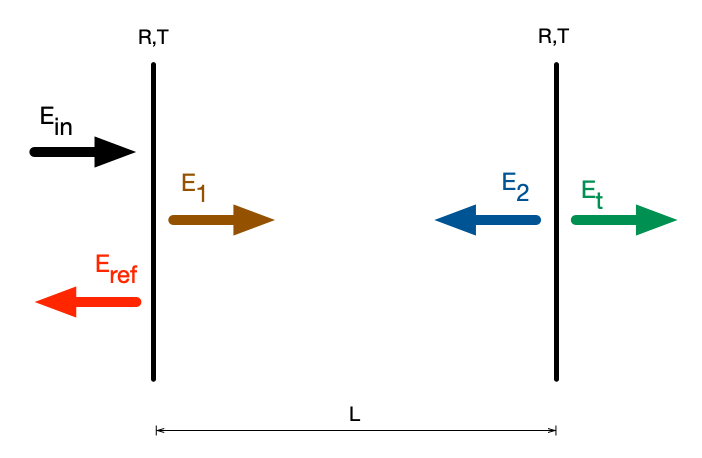
\includegraphics[width=.65\textwidth]{fp}
	\caption{Schematic representation of a \acrlong{fp} interferometer. $E_{\text{in}}$ is the incident electric field, $E_{\text{ref}}$ is the reflected electric field, $E_{\text{t}}$ is the transmitted electric field, $E_{1}$ is the intra-cavity electric field propagating from left to right, $E_{2}$ is the intra-cavity electric field propagating from right to left, $R$ and $T$ are the reflectivity and transmissivity of the mirrors and $L$ is the distance between them.}
	\label{fp}
\end{figure}

On figure \ref{fp-tf}, the transmissivity (right) and reflectivity (left) can be viewed. These graphs are made of peaks which are distant of the \gls{fsr} in the spectral domain. Recalling that $\text{FSR} = c/2nL$, one can see that the \gls{fsr} is linked to the length of the cavity, with $c$ the speed of light and $n$ the refractive index of the medium that could be present between the two mirrors ($nL$ is the optical path). The finesse $\mathcal{F}$ is related to the width of the peaks and depends on the reflectivity of the mirrors as $\mathcal{F} = 4R/(1-R)^2$. As the reflectivity of the mirrors tends to 1, the finesse tends to infinity, and the peaks get infinitely narrow. On the other hand, with a lower reflectivity, more energy can leak out of the cavity even outside the resonance condition. Seeing the broadening of the peaks as energy leakage will be useful when drawing a parallel between \gls{fp} and ring cavity interferometers.

\begin{figure}[h]
	\centering
	\begin{subfigure}{.5\textwidth}
		\centering
		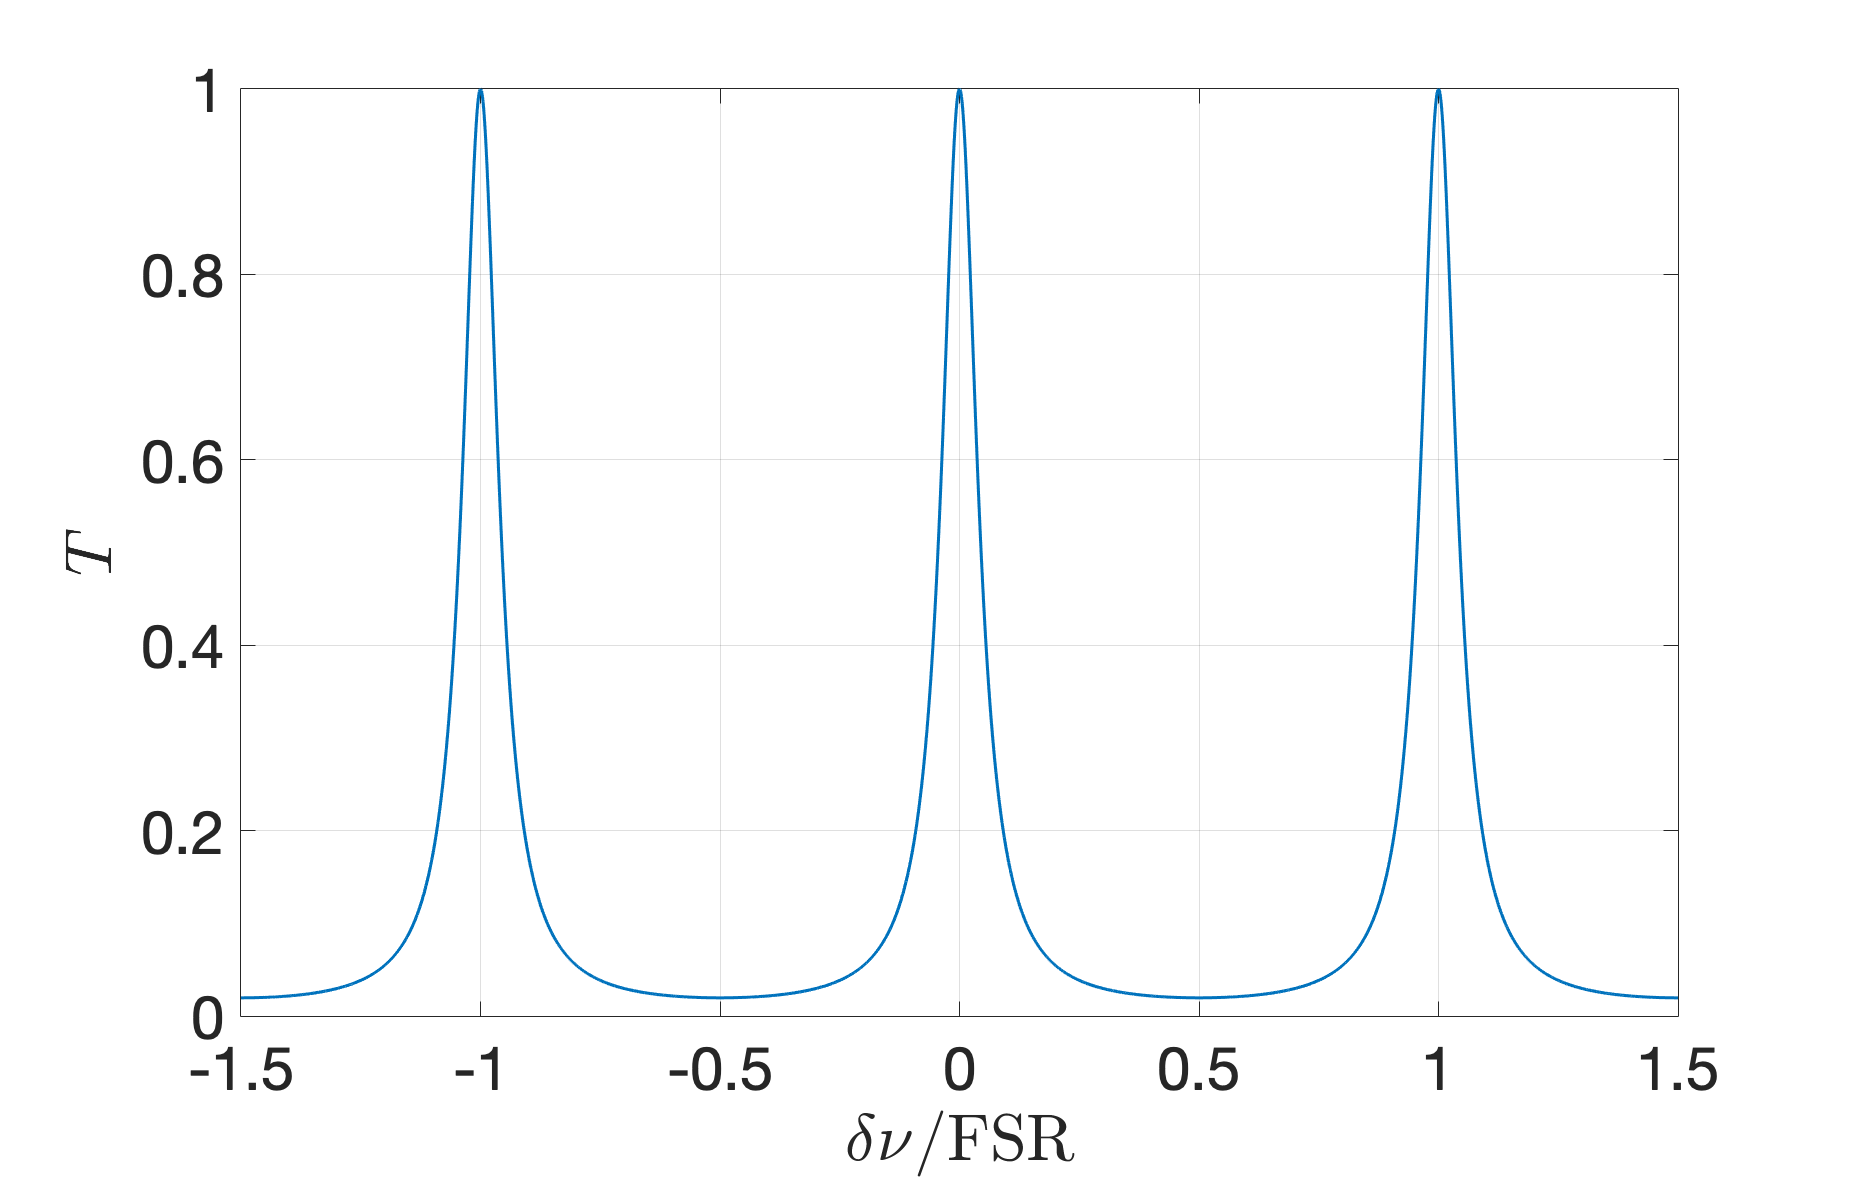
\includegraphics[width=\textwidth]{fp-trans-tf}
	\end{subfigure}%
	\begin{subfigure}{.5\textwidth}
		\centering
		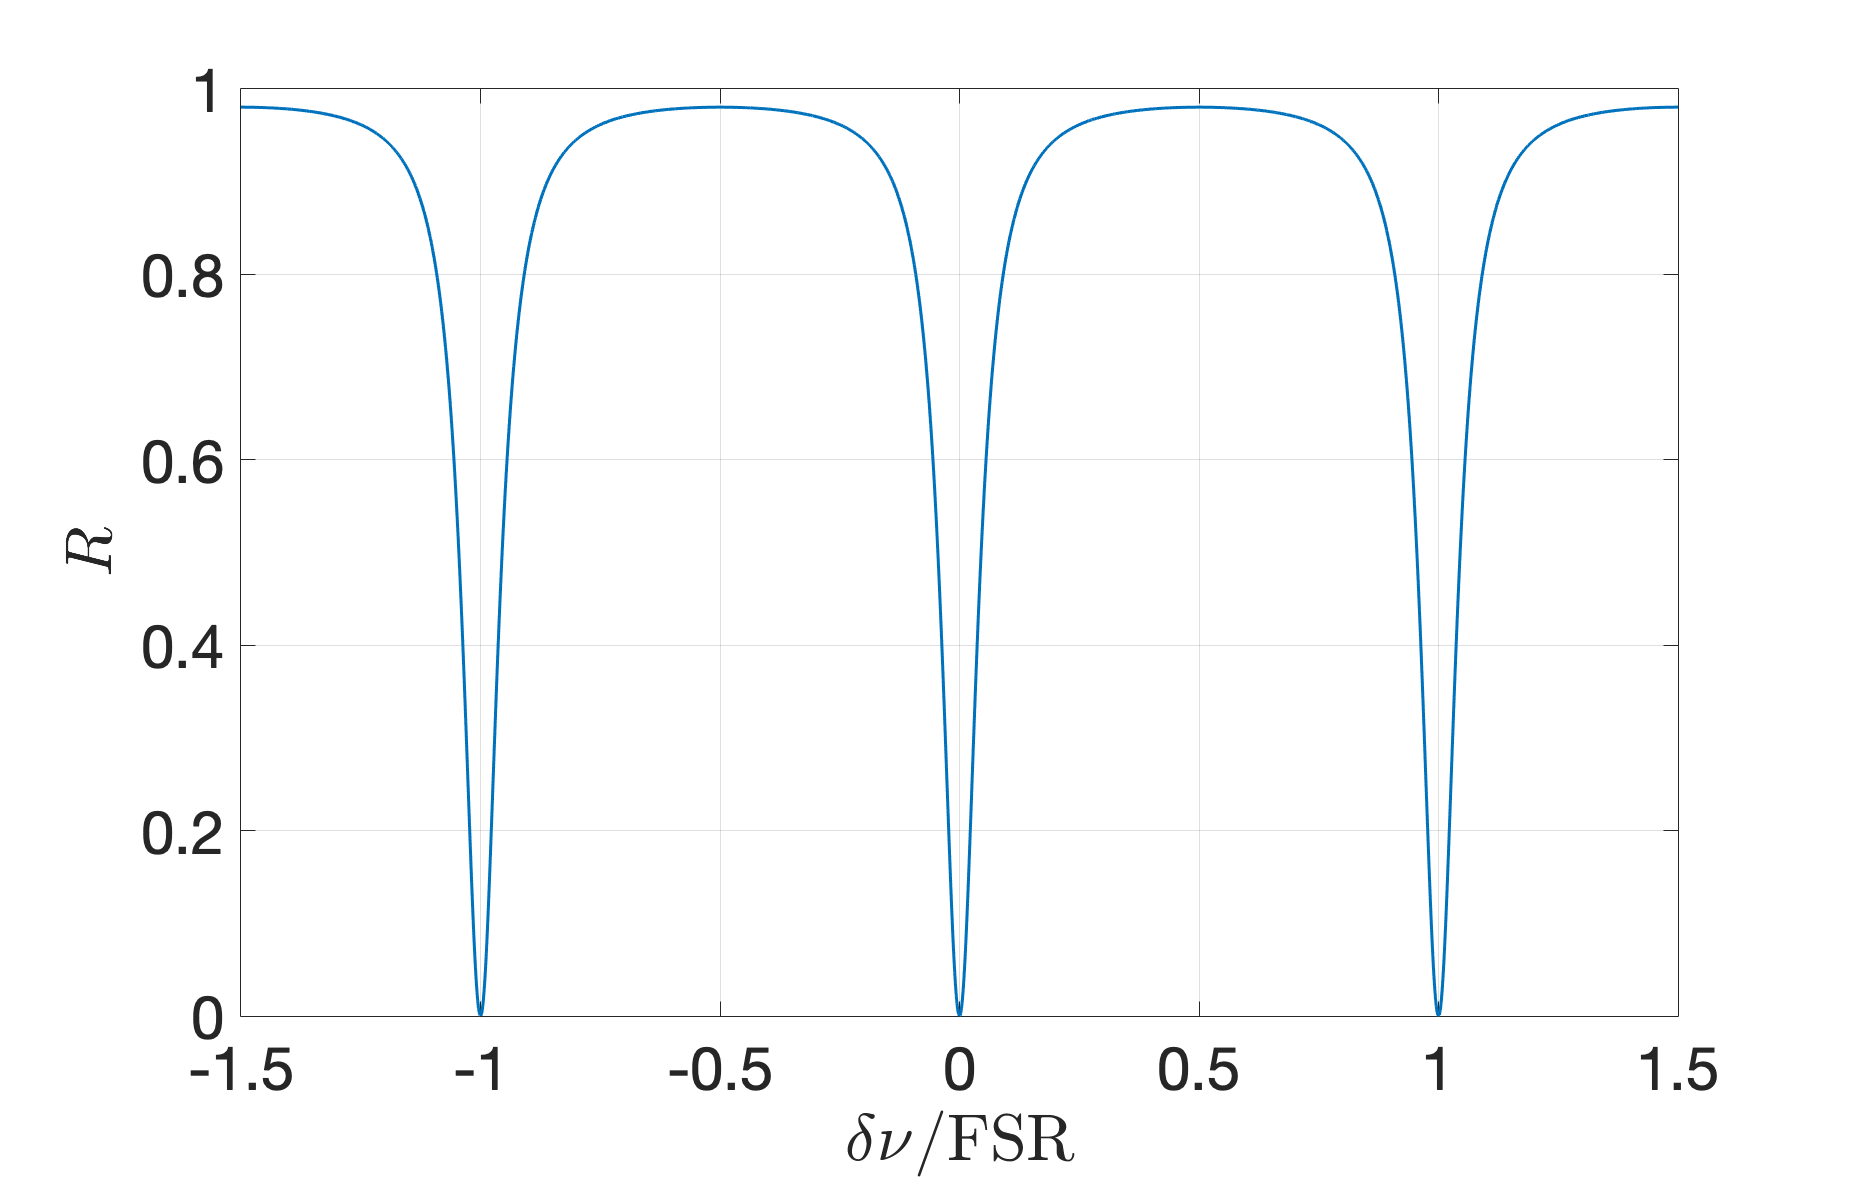
\includegraphics[width=\textwidth]{fp-ref-tf}
	\end{subfigure}
	\caption{Transmissivity $\mathcal{T}$ (left) and reflectivity $\mathcal{R}$ (right) of the cavity. Finesse $\mathcal{F}=50$. $\delta \nu$ denotes the deviation from a resonant frequency.}
	\label{fp-tf}
\end{figure}

Equation \eqref{transmissivity} and \eqref{reflectivity} indicate that $\mathcal{T}$ and $\mathcal{R}$ depend on $\omega/\text{FSR}$. This value can be rearranged as:

\begin{equation}
	\frac{\omega}{\text{FSR}} = kL = \phi
\end{equation}

Where $k$ is the wave number defined as $n \omega/c$ and $\phi$ is the phase acquired by the electric field when propagating along the cavity. Therefore, by measuring the transmitted or reflected power, one can gain information about the phase (modulo $\pi$, because the periodicity of $\mathcal{T}$ and $\mathcal{R}$ in the phase domain is $\pi$) of the electric field. This is the idea underlying interferometry.

%%% RING CAVITY %%%

\subsection{Ring cavity}

\label{subsec-ring-cavity}

A ring cavity exhibits the same behaviour as a \gls{fp} interferometer. The structure of a ring cavity interferometer is displayed on figure \ref{cavity_vs_fp}. This is a fibre-based setup in which the incident electric field $E_{\text{in}}$ penetrates the cavity from the left through a coupler. $E_{\text{ref}}$ denotes the electric field exiting the cavity and $E_1$ and $E_2$ refer to the fields entering and leaving the fibre loop, respectively. The nomenclature for the fields was chosen in such a way that the analogy with the \gls{fp} cavity can be understood. Indeed, one could see the coupler acting as the leftmost mirror from the figure \ref{fp}, and the fibre loop as the one on the right side because it turns $E_1$ into $E_2$ and dissipates energy through fibre losses, whereas for the mirror it was by leakage out of the cavity.

\begin{figure}[h]
	\centering
	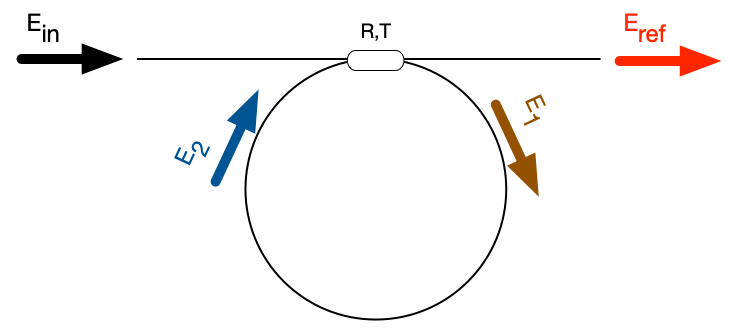
\includegraphics[width=.7\textwidth]{cavity_vs_fp}
	\caption{Schematic view of a ring cavity}
	\label{cavity_vs_fp}
\end{figure}

Because of the similarities between ring cavities and \glspl{fp}, the former show the same transmissivity and reflectivity as the latter. Therefore, by measuring the reflected power, one can determine the phase acquired by the electric field inside the cavity.

%%% Challenge %%%

\subsection{Challenge}

The basic principle of interferometry has been introduced through the presentation of the \gls{fp} interferometer, and in the discussion that followed, it has been shown that a ring cavity, such as the reservoir cavity studied in this thesis, can be used as an interferometer. Moreover, it has also been showed that $\mathcal{R}$ depends on the frequency (or wavelength) and on the length of the cavity and that the phase acquired by the incident electric field after one round trip could be determined by studying the reflected power.\\

In the reservoir cavity, many different wavelengths coexist because they encode the different neurons. Furthermore, after each round trip, the phase acquired by each neuron should be a constant, as shown on equation \eqref{model-reservoir}. Recalling the phase matrix $\mathbf{\Phi}$ defined in equation \eqref{phase-matrix}, the phase factor multiplying the $k^{\text{th}}$ neuron is given by $\Phi_{kk} = \exp{(i\phi_k)}$.	The phase $\phi_k$ is given by:

\begin{equation}
	\phi_k = \beta(\omega+k\Omega) L
\end{equation}

With $\beta$ the fibre wave number, $\omega+k\Omega$ the angular frequency of the $k^{\text{th}}$ neuron and $L$ the length of the fibre loop. Because $k\Omega \ll \omega$, the wave number can be Taylor expanded: 

\begin{equation}
	\beta(\omega+k\Omega) = \beta(\omega) + \left. \frac{\partial\beta}{\partial\omega}\right\rvert_\omega k\Omega + \mathcal{O}\left((k\Omega)^2\right)
\end{equation}

By rewriting $\beta(\omega)$ and $\partial\beta/\partial\omega\rvert_\omega$ as $\beta_0$ and $\beta_1$ as it is often done in the literature, the acquired phase is given by:

\begin{equation}
	\phi_k \approx \beta_0 L + k \beta_1 \Omega L = \phi_0 + k \phi_1
\end{equation}

This means that if $\phi_1$ is an integer multiple of $\pi$, the phase factor multiplying all the neurons will be the same up to a sign:

\begin{equation}
	e^{i(\phi_0+k\phi_1)} = e^{i\phi_0}e^{ikm\pi} =(-1)^{km} e^{i\phi_0}, \quad m \in \mathbb{Z}
\end{equation}

A periodicity of $\pi$ and not $2\pi$ is considered here, because as claimed before, an interferometer can only inform about a phase modulo $\pi$. Looking for an acquired phase equal to $\pi$ is the approximately the same as taking a modulation frequency $\Omega$ for the \gls{pm} which is an integer multiple of the \gls{fsr}. Indeed, by considering $\beta_1 \approx n/c$, one can find:

\begin{equation}
	\beta_1 \Omega L \approx \frac{\Omega n L}{c} = m\pi \longrightarrow \Omega \approx \frac{m\pi c}{n L} = m2\pi ~\text{FSR}
\end{equation}

This is a legitimate assumption given the fact that in the region of interest the curve of $\beta(\omega)$ computed using the Sellmeier relations \cite{Bruckner,malitson1965interspecimen} is very linear.\\

It is not critical to modulate the phase at an angular frequency $\Omega$ which is an integer multiple of the \gls{fsr}, the reservoir can in fact operate in different regimes. Those considerations were presented to better understand the physics underlying the phase management of the reservoir.\\

The main practical challenge regarding the reservoir concerns its stabilisation. The reservoir has to be stabilised because during its operation, external elements disturb it, which deteriorates the performances and even make it unusable in the worst case. The perturbations acting on the reservoir can come from various sources, such as mechanical constraints or temperature changes for example, and can induce a phase fluctuation. This is where interferometric stabilisation comes into play. Indeed, by measuring the power reflected by the reservoir, one can infer the current phase and take the appropriate action to maintain it at a setpoint. This can be achieved using classical regulation strategies, such as a \gls{pid} regulator. Elements of regulation will be presented later. Furthermore, this needs to be performed for all the neurons at the same time. This explains why different elements regarding the relative phases between the different neurons were discussed in the previous paragraph. Finally, the last technological difficulty associated to this scheme is the fact that the electric field used to stabilise the cavity is modulated in amplitude to carry the data to be processed by the reservoir. Indeed, a regulator struggles to differentiate a variation in the reflected power due to a phase fluctuation or to the modulation of the incident field.

%%%%%%%%%% EXPERIMENTAL SETUP %%%%%%%%%%

\section{Experimental setup}

In this section, the experimental setup employed to physically implement the \gls{wdm} \gls{prc} is presented. First, it is detailed based with the help of the schematic representation of figure \ref{exp-setup}. Then, technical data about the devices involved in the experiment are given.

\begin{figure}[h]
	\centering
	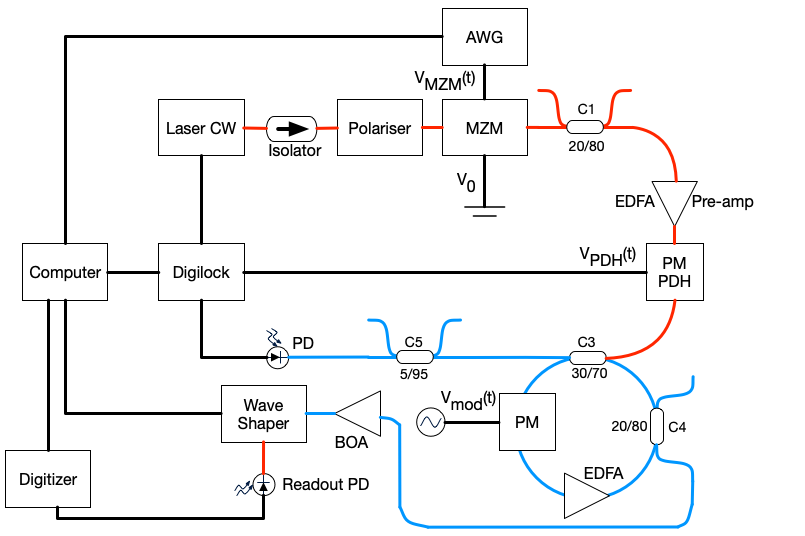
\includegraphics[width=\textwidth]{exp-setup}
	\caption{Schematic representation of the experimental setup for the \gls{wdm} reservoir computer experiment}
	\label{exp-setup}
\end{figure}

The setup presented here is mostly an update on the one presented on \cite{AkroutAkram2016Pprc}. On figure \ref{exp-setup}, electrical wires and single mode polarisation maintaining fibres are represented using black and coloured lines, respectively.  The light source exciting the setup is a narrow band continuous laser, which sends a single wavelength $\lambda_0 =$ 1555 nm to the reservoir. The light goes through an isolator that prevents any backward reflection towards the laser source and then enters a polariser that ensures that only one linear polarisation mode is present inside the setup. This needs to be done because the optoelectronic devices involved in the experiment, such as the \gls{mzm} and the \glspl{pm}, are polarisation dependent. The electric field then enters a \gls{mzm} which is driven by the time dependent voltage $V_{\text{MZM}}(t)$. This signal is generated by an \gls{awg} based on the input time series $u(n)$ sent by the computer running the experiment. Since the transfer function of the \gls{mzm} is nonlinear, the signal $V_{\text{MZM}}$ can be precompensated in order to counteract the nonlinearity. Without precompensation, the voltage $V_{\text{MZM}}(t)$ is simply given by $\beta \tilde{u}(t)$, with $\beta$ the input gain $\in [0,1]$ and $\tilde{u}(t)$ the \textit{sample and hold} version of $u(n)$ already introduced in the previous chapter. A bias tension $V_0$ can also be applied to the \gls{mzm} to change its average transparency. The transfer function of the \gls{mzm} is given by :

\begin{equation}
	\sin{ \left(\frac{\pi}{2} \left(\frac{V_{\text{MZM}}(t)}{V_{\pi,\text{RF}}} + \frac{V_0}{V_{\pi, \text{DC}}} \right) \right)}
\end{equation}

With $V_{\text{MZM}} \in [-\beta V_{\pi,\text{RF}},\beta V_{\pi,\text{RF}}]$, and $V_{\pi,\text{RF}}$ and $V_{\pi,\text{DC}}$ the dynamic and static characteristic voltages of the \gls{mzm}, respectively. The modulated electric field is then pre-amplified using an \gls{edfa}, and undergoes a first phase modulation. This is required to be able to implement the \gls{pdh} stabilisation technique, which is an advanced cavity stabilisation scheme that is described with greater length in section \ref{sec-pdh}. The \gls{pm} is driven by the alternative voltage $V_{\text{PDH}} = A_{\text{PDH}} \sin{(\Omega_{\text{PDH}}t)}$ supplied by the \textit{Toptica Digilock 110} feedback controller denoted "Digilock" on the figure. This device handles every aspects related to the stabilisation of the reservoir, which is why it needs to be connected to the photodiode "PD" and to the laser, which are both involved in the regulation of the cavity (see later). The electric field then enters the reservoir through the coupler "C3". The reservoir cavity is made of the fibres of the different couplers and is around \SI{18}{m} long. At this point, the colour used to represent the optical fibres changes from red to blue to indicate that inside the reservoir, several wavelengths are present whereas before the coupler there was only one. Inside the reservoir, the \gls{pm} is used to mix the different frequencies and is driven by an external alternative voltage $V_{\text{mod}}(t) = A_{\text{mod}} \sin{ (\Omega_{\text{mod}} t)}$. To allow a clear distinction between the different sidebands without degrading the achievable modulation depth, the modulation frequency $\pulsefreq{\Omega_{\text{mod}}}$ is around 20 GHz. This allows the existence of 13 neurons inside the cavity (6 sidebands on both sides of the central frequency) with wavelengths going from \SIrange{1.554}{1.556}{\micro\metre}. The \gls{pm} introduces insertion losses that are compensated using the \gls{edfa}, whose pump current is adjusted to tune the feedback gain $\alpha$ that appears in equation \eqref{model-reservoir}. The electric field exiting the reservoir at the level of the coupler "C3" towards the photodiode "PD" is the reflected field, according to what was discussed in section \ref{subsec-ring-cavity}. The electric field finally illuminates the photodiode "PD", which produces a voltage proportional to its intensity. This measured signal enters the Digilock where it is compared to a reference. Based on the deviation between those two values, the Digilock outputs a control voltage that is applied to a piezoelectric crystal inside the laser cavity and that modifies its emission wavelength. The output of the reservoir exits the cavity thought the coupler "C4" and is amplified by a \gls{soa} called "BOA" for Boost Optical Amplifier to improve the \gls{snr}. A demultiplexing scheme allowing to obtain the value of each individual neuron at the same time has not been implemented yet. To overcome this limitation, the adjustable band-pass filter denoted "Wave Shaper" is used to record the evolution of only one neuron at a time. This implies that if one wants to compute the output of the reservoir $y(n)$, one has to run the same experiment once for each of the neuron, to program the Wave Shaper to filter out all the other sidebands and to save its evolution on the computer. Once this has been done, $y(n)$ can be reconstructed. As far as the learning procedure is concerned, it follows the same procedure as the one previously described, but modified to take this sequential measurements of the neurons into account. In terms of the devices used to perform this task, the photodiode "Readout PD" measures the intensity of each of the filtered neuron, and the "Digitizer" handles the conversion between continuous time dependent signals into time series usable by the computer. To conclude this description of the experimental setup, one should note that even though the couplers "C1" and "C2" seem useless, they are used in practice to monitor the electric fields when modifications are made to the optical table, and that the AWG, Digilock, Wave Shaper and Digitizer are all controlled by the computer. The technical specifications of the devices used in the experiment can be found in appendix \ref{app-data}.

%%%%%%%%%% CHARACTERISATION OF THE RESERVOIR %%%%%%%%%%

\section{Characterisation of the reservoir}

To be able to develop a reliable stabilisation scheme for the reservoir, some of its characteristics need to be studied as a preliminary work. First, one can gain important insights by modelling the transfer function of the reservoir. In this context, the transfer function is simply the reflectivity of the cavity. However, given the fact that the reservoir is a more complex ring cavity than the one depicted in section \ref{subsec-ring-cavity}, it will not exhibit the exact same behaviour as the one of a \gls{fp} cavity as displayed on figure \ref{fp-tf}. A mathematical model is first derived and the results it provides are compared to experimental transfer functions. After that, the experimental study of the effective losses is tackled. The effective losses are used in the model to take into account the fibre losses, the insertion losses of the \gls{pm} and the gain of \gls{edfa} using only one factor. Finally, an empirical relation between the modulation amplitude driving the intra-cavity \gls{pm} and its modulation depth is determined experimentally.

%%% TRANSFER FUNCTION OF THE CAVITY %%%

\subsection{Transfer function of the cavity}

As already claimed, in the context of cavity stabilisation, the transfer function is the reflectivity. When operating the reservoir, the reflected power which is proportional to the intensity of the electric field reflected by the cavity gives an indication on the phase of the field inside it, which implies that the regulation procedure relies on the measurement of this signal. \\

On figure \ref{schematic_reservoir}, the reservoir is represented with the different electric fields that turn out to be useful when studying the transfer function. The colour code for the fibres is the same as the one used previously. The incident electric field $\efield{in}$ enters the cavity through a coupler from the top left optical fibre. Inside the cavity, it is amplified by the \gls{edfa} and then is phase modulated. After that, a portion of the electric field exits the cavity through the coupler C4 to be read out. The light inside the cavity finally terminates its round trip.

\begin{figure}[h]
	\centering
	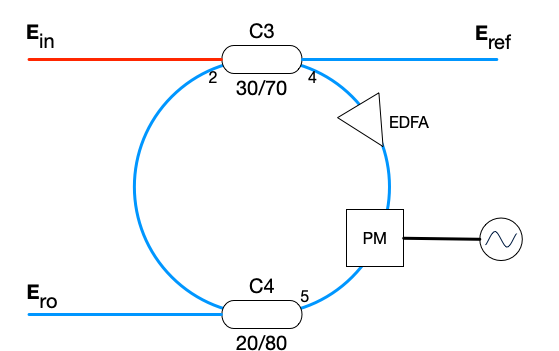
\includegraphics[width=.7\textwidth]{reservoir}
	\caption{Schematic representation of the reservoir}
	\label{schematic_reservoir}
\end{figure}

% MATHEMATICAL MODEL %

\subsubsection{Mathematical model}

In this section, a mathematical model for the transfer function is derived. To do so, the formalism introduced in section \ref{subsec-reservoir-model} needs to be used. This can be done because the basis vectors where chosen such that a neurons state vector $\mathbf{x}$ is formally equal to an electric field. Therefore, one should pay attention to the fact that when referring the a vectorial electric field $\mathbf{E}$, it denotes an electric field expressed in the abstract basis $\{ \hat{\mathbf{e}}_j | \hat{\mathbf{e}}_j = \exp{ (i (\omega+j\Omega_{\text{mod}}t)}, ~j\in [-\eta, \eta ] \}$ instead of the usual physical space $\{\mathbf{1}_x, \mathbf{1}_y,\mathbf{1}_z \}$.\\

The transfer function $\mathbf{R}$ is defined as the link between the incident and reflected electric fields:

\begin{equation}
	\efield{ref} = \mathbf{R} ~\efield{in}
\end{equation}

Given the vectorial nature of $\efield{ref}$ and $\efield{in}$, the transfer function is in fact a transfer matrix in this particular context. Recalling that the laser only emits light at the center wavelength, the incident field $\efield{in}$ is given by:

\begin{equation}
	\efield{in} = E_0 \hat{\mathbf{e}}_0
\end{equation}

With $E_0$ being an arbitrary complex amplitude. Given the properties of the coupler C3, one finds:

\begin{equation}
	\begin{bmatrix}
		\efield{ref}\\
		\efield{4}
	\end{bmatrix} = \begin{bmatrix}
		\epsilon_1 & i\sqrt{1-\epsilon_1^2} \\
		i\sqrt{1-\epsilon_1^2} & \epsilon_1
	\end{bmatrix}
	\begin{bmatrix}
		\efield{in}\\
		\efield{2}
	\end{bmatrix} 
\end{equation}

Which yields to the following expression for the reflected field:

\begin{equation}
	\efield{ref} = \epsilon_1 \efield{in} + i \sqrt{1-\epsilon_1^2} \efield{2}
	\label{eq-ref}
\end{equation}

Let us now express $\efield{2}$ as a function of $\efield{in}$ to close the system. Using the transfer matrix of the coupler C4, $\efield{2}$ reads :

\begin{equation}
	\begin{bmatrix}
		\efield{2}\\
		\efield{ro}
	\end{bmatrix} = e^{-\gamma L} \begin{bmatrix}
		\epsilon_2\\
		\sqrt{1-\epsilon_2^2}
	\end{bmatrix} \efield{5} \Longrightarrow \efield{2} = \epsilon_2 e^{-\gamma L} \efield{5}
\end{equation}

With $\gamma$ the effective losses coefficient and $L$, the length of the reservoir. Since the system is in a linear regime, the position of the coupler C4 in the cavity has no influence on the losses and on the phase. By defining $\xi \in [0,1]$ as the variable indicating the relative position of the \gls{pm} inside the cavity ($\xi = 0$ if it is at the beginning of the cavity, $\xi=1$ if it is at the end). The phase acquired  by the electric field inside the reservoir is now dependent on the position of the \gls{pm}. This leads to the definition of two new matrices $\mathbf{\Phi}_\xi$ and $\mathbf{\Phi}_{1-\xi}$, which are based on the phase matrix $\mathbf{\Phi}$. They are diagonal matrices, expressed as:

\begin{align}
	\Phi_{\xi,nn} &= \exp{ \left(i \beta (\omega+n\Omega_{\text{mod}}) \xi L \right)} \nonumber \\
	\Phi_{1-\xi,nn} &= \exp{ \left(i \beta (\omega+n\Omega_{\text{mod}}) (1-\xi) L \right)}
\end{align}

With $\beta (\omega+n\Omega_{\text{mod}})$ the dispersion relation of the fibre evaluated at the frequency of the $n^{\text{th}}$ neuron. Recalling the coupling matrix of the \gls{pm} $\mathbf{J}$, one can rewrite $\efield{5}$ as a function of $\efield{4}$:

\begin{equation}
	\efield{5} = \mathbf{\Phi}_{1-\xi} \mathbf{J} \mathbf{\Phi}_\xi \efield{4}
\end{equation}

Using the transfer matrix of the coupler C3, one can express $\efield{4}$ as a function of $\efield{in}$ and $\efield{2}$:

\begin{equation}
	\efield{4} = i\sqrt{1-\epsilon_1^2} \efield{in} + \epsilon_1 \efield{2}
\end{equation}

This yields to a closed equation to determine $\efield{2}$:

\begin{align}
	\efield{2} &= i\sqrt{1-\epsilon_1^2} \epsilon_2 e^{-\gamma L} \mathbf{\Phi}_{1-\xi} \mathbf{J} \mathbf{\Phi}_\xi \efield{in} + \epsilon_1 \epsilon_2 e^{-\gamma L} \mathbf{\Phi}_{1-\xi} \mathbf{J} \mathbf{\Phi}_\xi \efield{2} \nonumber \\
	\hookrightarrow \efield{2} &= i \sqrt{1-\epsilon_1^2} \epsilon_2 e^{-\gamma L} \left( \mathbf{I} - \epsilon_1 \epsilon_2 e^{- \gamma L} \mathbf{\Phi}_{1-\xi} \mathbf{J} \mathbf{\Phi}_\xi \right)^{-1} \mathbf{\Phi}_{1-\xi} \mathbf{J} \mathbf{\Phi}_\xi \efield{in}
\end{align}

Now that $\efield{2}$ has been determined, it is easy to compute $\efield{ref}$ using equation \eqref{eq-ref}:

\begin{align}
	\efield{ref} &= \epsilon_1 \efield{in} - (1-\epsilon_1^2) \epsilon_2 e^{-\gamma L} \left( \mathbf{I} - \epsilon_1 \epsilon_2 e^{- \gamma L} \mathbf{\Phi}_{1-\xi} \mathbf{J} \mathbf{\Phi}_\xi \right)^{-1} \mathbf{\Phi}_{1-\xi} \mathbf{J} \mathbf{\Phi}_\xi \efield{in} \nonumber \\
	\hookrightarrow \efield{ref} &= (\epsilon_1 \mathbf{I} - (1-\epsilon_1^2) \epsilon_2 e^{-\gamma L} \left( \mathbf{I} - \epsilon_1 \epsilon_2 e^{- \gamma L} \mathbf{\Phi}_{1-\xi} \mathbf{J} \mathbf{\Phi}_\xi \right)^{-1} \mathbf{\Phi}_{1-\xi} \mathbf{J} \mathbf{\Phi}_\xi) \efield{in}
\end{align}

This last equality reveals the expression of the transfer matrix $\mathbf{R}$:

\begin{equation}
	\boxed{\mathbf{R} = \epsilon_1 \mathbf{I} - (1-\epsilon_1^2) \epsilon_2 e^{-\gamma L} \left( \mathbf{I} - \epsilon_1 \epsilon_2 e^{- \gamma L} \mathbf{\Phi}_{1-\xi} \mathbf{J} \mathbf{\Phi}_\xi \right)^{-1} \mathbf{\Phi}_{1-\xi} \mathbf{J} \mathbf{\Phi}_\xi}
\end{equation}

Even if this result is interesting, it cannot be measured directly since it involves electric fields instead of intensities. What is measured using a \gls{pd} is the reflectivity $\mathcal{R}$ linking the incident intensity to the reflected intensity. Recalling that the incident electric field is given by $\efield{in} = E_0 \hat{\mathbf{e}}_0$, the reflected electric field is given by:

\begin{equation}
	\efield{ref} = \mathbf{R}~\efield{in} = E_0\sum_{n=-\eta}^\eta R_{n,0} \hat{\mathbf{e}}_n
\end{equation}

The sum in this formula is expressed using the numbering introduced in section \ref{subsec-reservoir-model} which is more natural for this kind of situation. As a reminder, instead of going through the indices from 1 to $N$, this alternative notation goes from $-\eta$ to $\eta$, with index 0 referring to the central neuron. Thus, the above equation basically means that $\efield{ref}$ is equal to $E_0$ multiplying the central column of $\mathbf{R}$.\\

The reflected intensity is given by:

\begin{equation}
	|\efield{ref}|^2 = |E_0|^2 \left(\sum_{n=-\eta}^\eta R_{n,0} \hat{\mathbf{e}}_n \right) \left(\sum_{m=-\eta}^\eta R_{m,0}^* \hat{\mathbf{e}}_m^* \right)
\end{equation}

This expression seems complicated at first sight, but it can be simplified by putting forward an experimental argument. First, let us consider the product $\hat{\mathbf{e}}_n \cdot \hat{\mathbf{e}}_m^*$, which is equal to $\exp{(i(n-m)\Omega_{\text{mod}}t)}$. If $m=n$, then the product is equal to one and the term $|R_n,0|^2$ has to be taken into account in the sum. On the other hand, if $m\neq m$, then product corresponds to a beating of the intensity at frequency $(n-m)\pulsefreq{\Omega_{\text{mod}}}$, which is an integer number of times approximately 20 GHz. However, as can be seen in the appendix \ref{app-data}, the bandwidth of the \gls{pd} is limited to 120 MHz. Therefore the \gls{pd} is not able to resolve the beating waves, which implies that when $m=n$, the signals do not contribute to the sum. This yields to a simplified version of the reflected intensity:

\begin{equation}
	|\efield{ref}|^2 = |E_0|^2 \sum_{n=-\eta}^\eta |R_{n,0}|^2
\end{equation}

The reflectivity of the reservoir is finally given by:

\begin{equation}
	\mathcal{R} = \sum_{n=-\eta}^\eta |R_{n,0}|^2
\end{equation}

Note that this model is solely valid when considering the evolution of the reservoir at time scales much larger than $2\pi / \omega$. This assumption ensures that one is working in a stationary regime with respect to the oscillations of the electric field.

% EXPERIMENTAL RESULTS %

\subsubsection{Experimental results}

The adequacy of the analytical model just derived is assessed by comparing its predictions to experimental data. To capture data concerning transfer functions, one performs a \textit{sweep} using the Digilock. As already explained, the Digilock is connected to a piezoelectric crystal controlling the emission wavelength of the laser, whose shift is proportional to the applied tension. As a reminder, the transfer function is the reflectivity $\mathcal{R}$ as a function of $\omega$, therefore one needs to be able to scan the frequency domain. The sweep procedure allows to do it by applying a triangular periodic voltage to the piezoelectric, which leads to a similar evolution of the emission wavelength of the laser. The frequency and amplitude of this signal are controlled by the Digilock interface. After doing this trick, one can plot the reflected power as a function of the time to observe its shape.\\

To relate the theoretical curves to raw data, one should express the link between the time and the angular frequency. Using a first order Taylor approximation, the angular frequency variation reads:

\begin{equation}
	\delta \omega = -\frac{2\pi c}{\lambda_0^2} \delta \lambda
\end{equation}

With $\lambda_0$ the central wavelength (1555 nm). In appendix \ref{app-data}, one can find that the piezoelectric tuning characteristic is equal 0.1 pm/V at a sweeping frequency of \SI{100}{\Hz}. Let us denote this value by $\alpha$ and let us call $\beta$ the slope of the triangular voltage as a function of the time, which depends on the settings of the sweep. Multiplying those two constants provides a proportionality indicating the range of wavelengths spanned per unit of time. This yields to a link between time and angular frequency:

\begin{equation}
	\omega = - \alpha \beta \frac{2 \pi c}{\lambda_0^2} t
	\label{eq-omega-vs-t}
\end{equation}

Below, comparisons between simulations and experimental data are shown for three different regimes. Since the theoretical reflectivity $\mathcal{R}$ is a ratio, it is comprised between 0 and 1. Therefore, it had to be rescaled in order to be compared with the reflected powers measured by the \gls{pd}.

\paragraph{First sideband at resonance} If the central neuron is at resonance, this means that $\omegamod$ is chosen such that the first sideband is at resonance as well. In other words, $\pulsefreq{\omegamod}$ is an integer number of times the \gls{fsr} of the cavity. This is displayed on figure \ref{tf_0}.

\begin{figure}
	\centering
	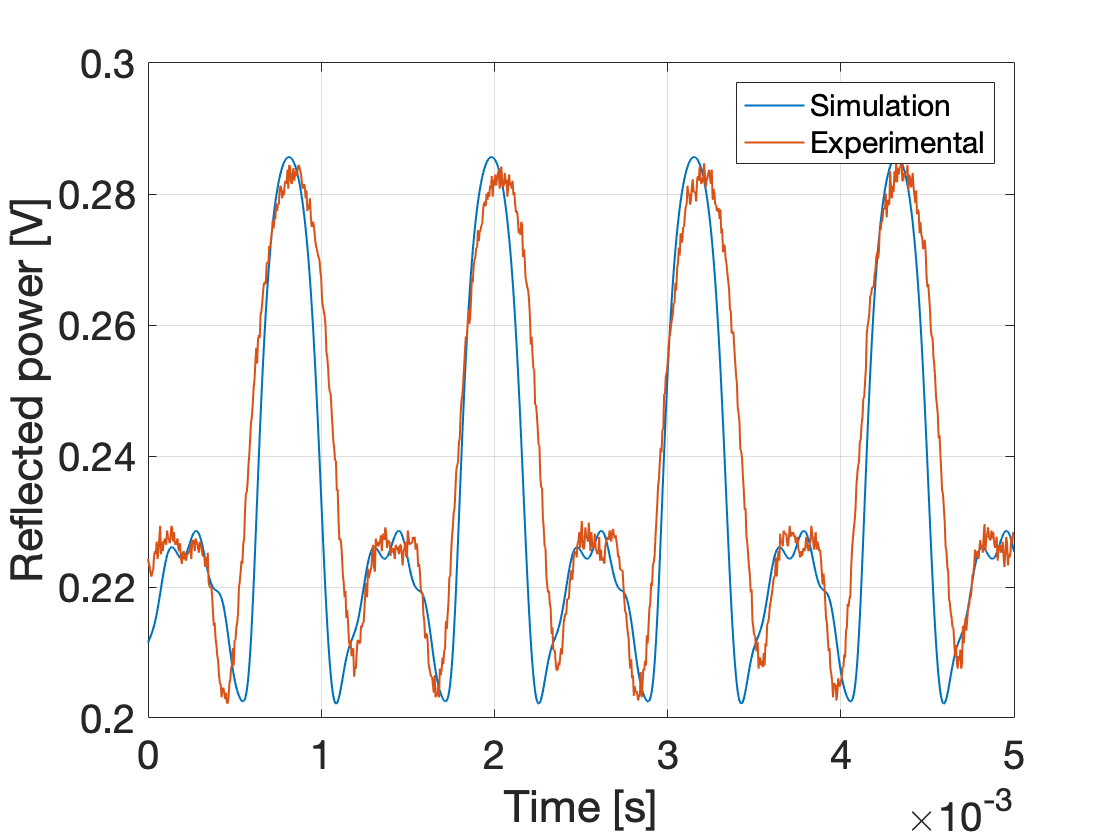
\includegraphics[width=.7\textwidth]{exp-tf-reservoir/tf_0.png}
	\caption{Reflected power [V] as a function of the time [s] during a sweep of the Digilock. First sideband at resonance. $\Omega_{\text{mod}}$ = 19.99 GHz, modulation depth $m$ = 2, $\gamma = 0.0126~\text{m}^{-1}$}
	\label{tf_0}
\end{figure}

\paragraph{First sideband halfway between resonance and anti-resonance} $\omegamod$ is tuned such that $\pulsefreq{\omegamod}$ is an odd number of times the quarter of the \gls{fsr}. The experimental results are given on the figure \ref{tf_25}.

\begin{figure}
	\centering
	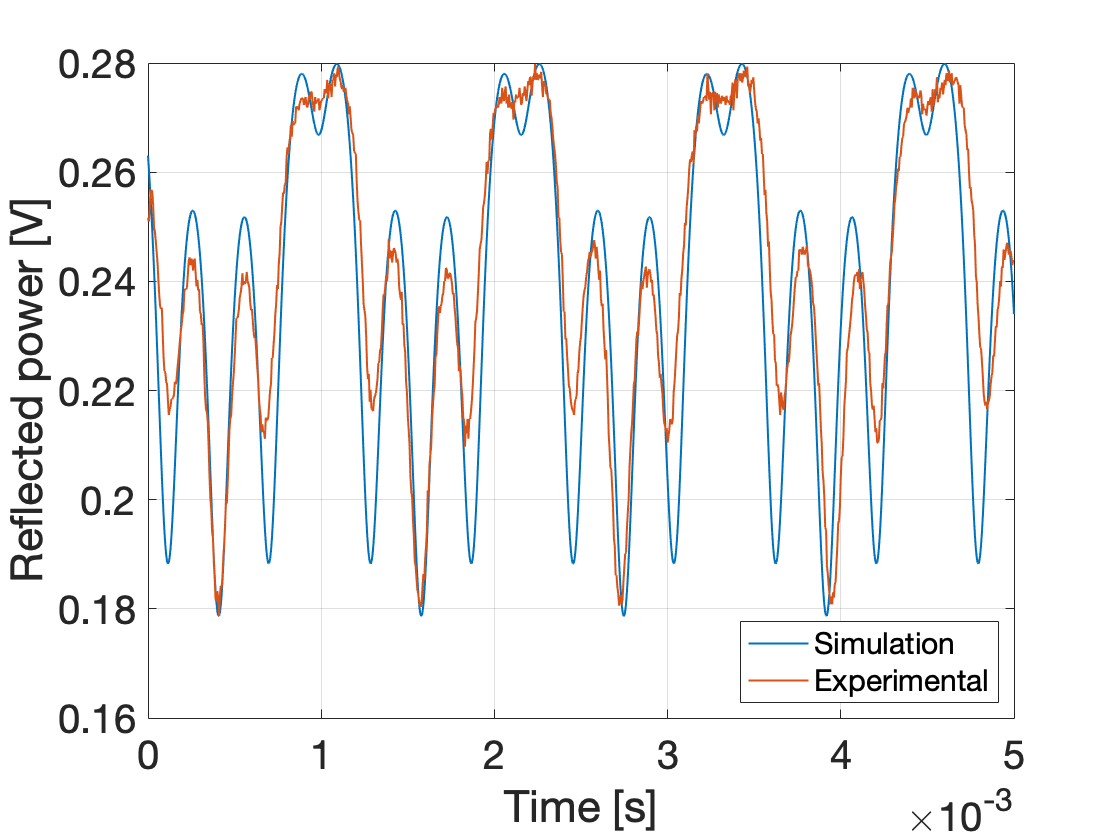
\includegraphics[width=.7\textwidth]{exp-tf-reservoir/tf_25.png}
	\caption{Reflected power [V] as a function of the time [s] during a sweep of the Digilock. First sideband halfway between resonance and anti-resonance. $\Omega_{\text{mod}}$ = 19.9997 GHz, modulation depth $m$ = 2, $\gamma = \SI{0.0126}{\per\metre}$.}
	\label{tf_25}
\end{figure}

\paragraph{First sideband at anti-resonance} $\pulsefreq{\omegamod}$ is an odd number of times half of the \gls{fsr}. The graphs are depicted on the figure \ref{tf_50}.\\

\begin{figure}
	\centering
	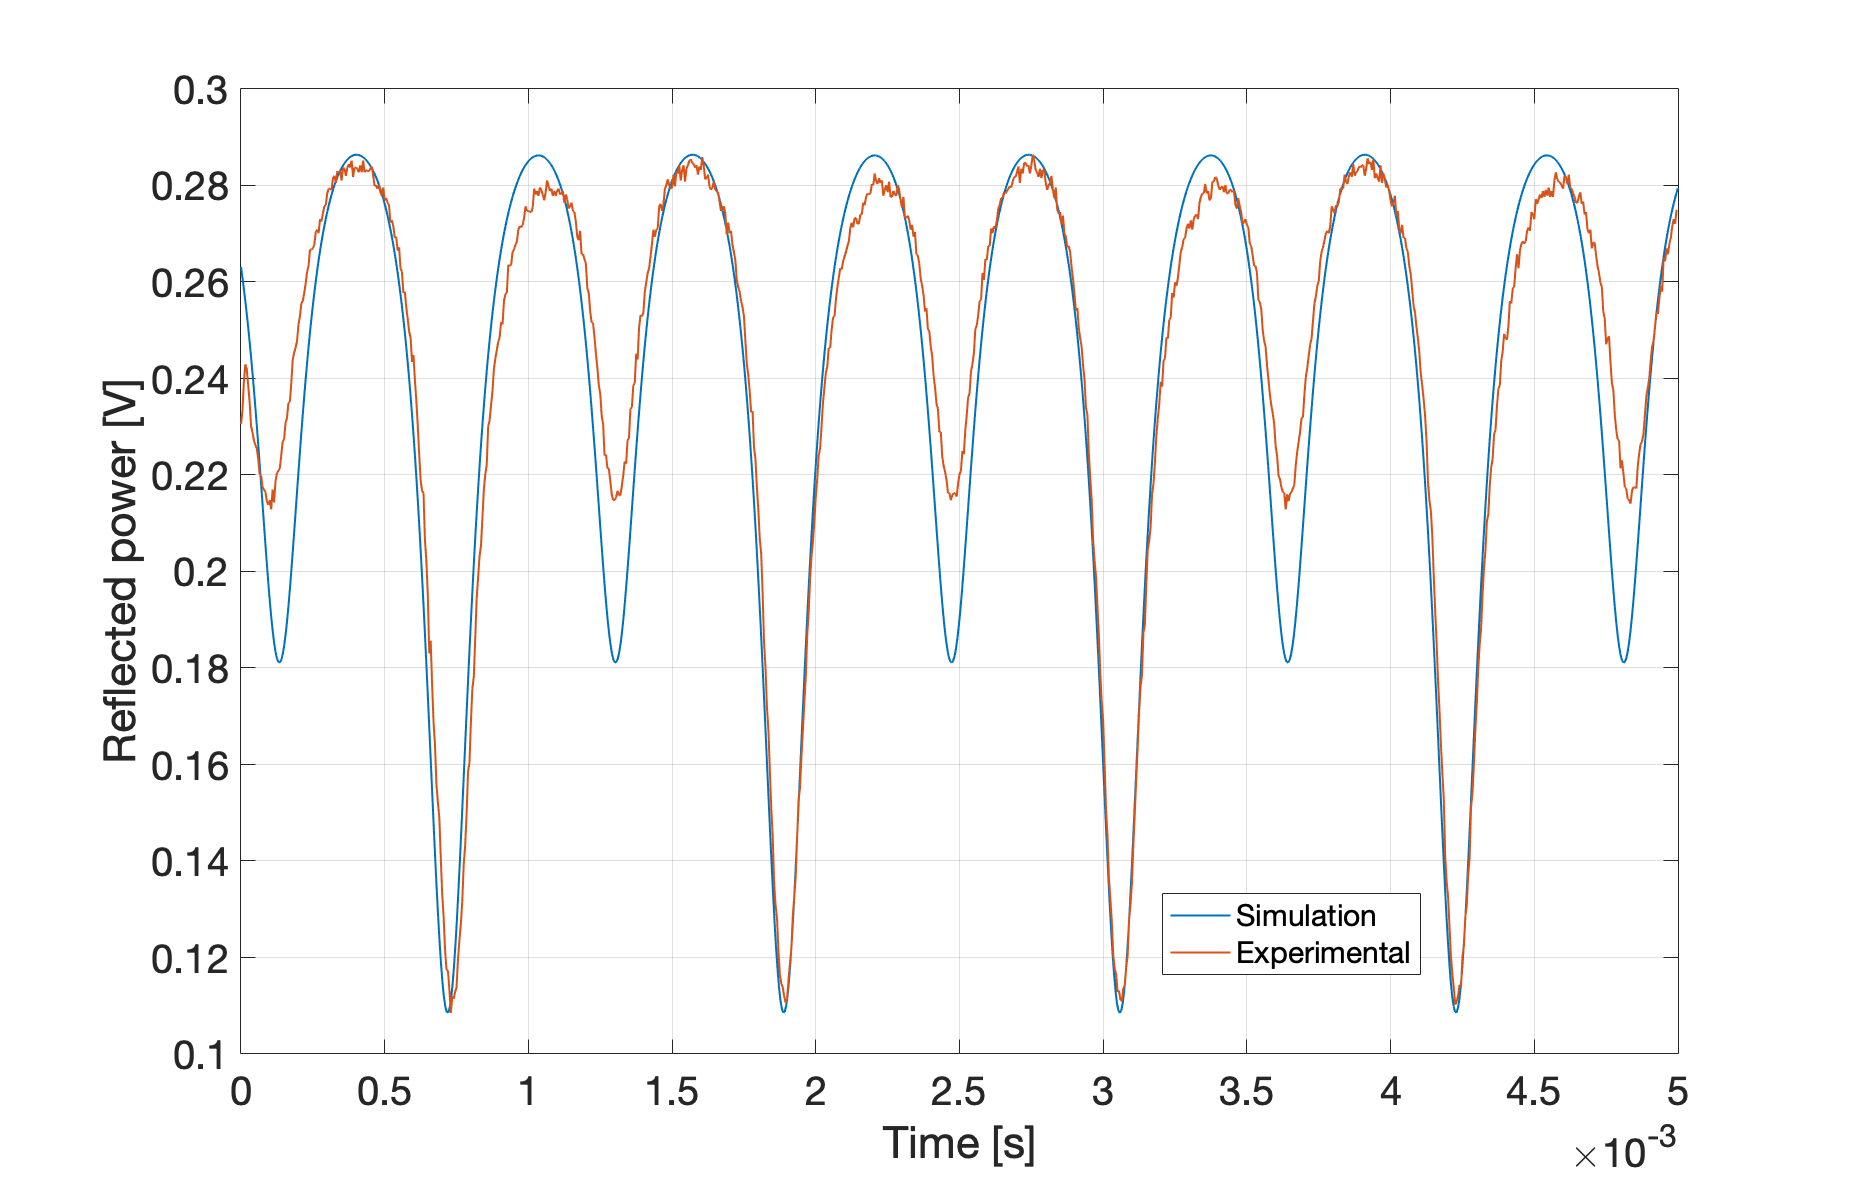
\includegraphics[width=.7\textwidth]{exp-tf-reservoir/tf_50.png}
	\caption{Reflected power [V] as a function of the time [s] during a sweep of the Digilock. First sideband at anti-resonance. $\Omega_{\text{mod}}$ = 19.9997 GHz, modulation depth $m$ = 2, $\gamma = \SI{0.0126}{\per\metre}$.}
	\label{tf_50}
\end{figure}

One those graphs, one can see that the transfer function highly depends on the modulation frequency, and more specifically, on the position of the first sideband. Even though the experimental adequacy is not perfect, it is sufficient to have a qualitative idea of the behaviour of the reservoir. It also allows to experimentally deduce its \gls{fsr} by measuring the temporal periodicity of the reflectivity, and then to translate in the frequency domain using equation \eqref{eq-omega-vs-t}.

\begin{equation}
	\Delta t = \SI{1.155}{\milli\second} \Longrightarrow \text{FSR} \approx  \alpha \beta \frac{c}{\lambda_0^2} \Delta t  \approx \SI{11.5}{\mega\hertz}
\end{equation}

Recalling that the \gls{fsr} for a ring cavity is given by\footnote{This comes from the fact that the resonance condition is not exactly the same as \gls{fp} for a ring cavity: $\beta L = 2m\pi$ instead of $\beta L = m \pi$ for a \gls{fp}}:

\begin{equation}
	\mathrm{FSR} = \frac{c}{nL}
\end{equation}

Using this formula, one can compute the length of the cavity: $L=\SI{18.33}{\metre}$.

As a final remark, the relative position of the \gls{pm} inside the cavity (controlled using the variable $\xi$) does not seem to have an influence on the shape of the transfer function.

%%% EFFECTIVE LOSSES %%%

\subsection{Effective losses}

Given the model derived, the only physical quantity that cannot be known from a simple inspection of the data sheets are the effective losses $\gamma$. They arise due to the conjugated effects of the fibre losses, the insertion loss of the intra-cavity \gls{pm} and the gain of the \gls{edfa}, and in the same way that the use of a lower reflectivity mirror induced a worse finesse for a \gls{fp}, the effective losses lead to a broadening of the resonance peaks. Although their value could have been derived analytically, it has been chosen to determine it experimentally. To do so, a least square fit is performed. Basically, this means that one compares an experimental curve with an analytical one, for which the value of $\gamma$ is not fixed. The deviation between those two curves is therefore a function of $\gamma$, and can be minimised. Mathematically speaking, the experimental effective losses $\tilde{\gamma}$ are given by:

\begin{equation}
	\tilde{\gamma} = \underset{\gamma}{\mathrm{argmin}} \sum_{i=1}^T (\mathcal{R}_i - \mathcal{R}(t_i;\gamma))^2
\end{equation}

Where $T$ is the total number samples, $\mathcal{R}_i$ is the measured reflected power for the $i^{\text{th}}$ sample and $\mathcal{R}(t_i;\gamma)$ is the theoretical rescaled reflectivity evaluated at $t=t_i$ and $\gamma$, which is the time corresponding to the $i^{\text{th}}$ sample and the effective losses, respectively. On figure \ref{eff-losses}, one can see the result of this optimisation. It was performed on the reservoir without phase modulation because it is assumed that the insertion losses do not dependent on whether a phase modulation is going on. The effective losses that were determined using this procedure read:

\begin{equation}
	\gamma = \SI{0.0126}{\per\metre}
\end{equation}

\begin{figure}
	\centering
	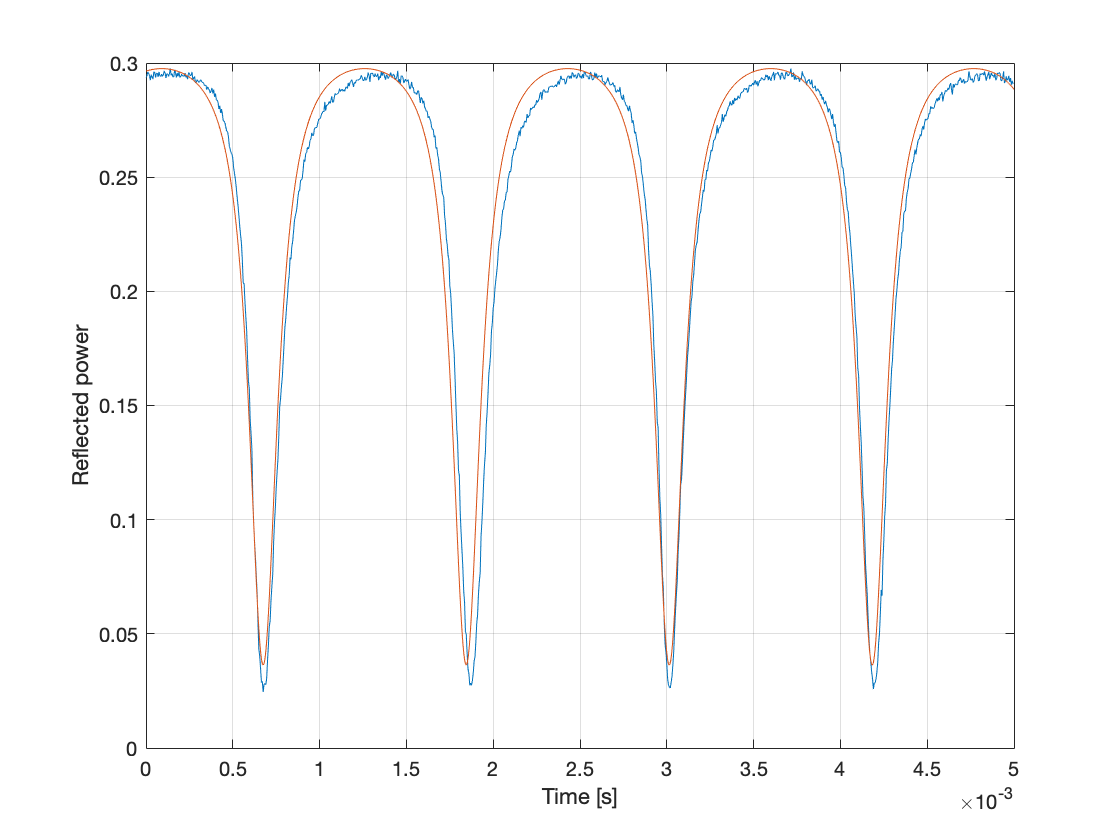
\includegraphics[width=.7\textwidth]{exp-tf-reservoir/eff_losses.png}
	\caption{Reflected power [V] as function of the time [s] during a sweep of the Digilock, no intra-cavity phase modulation, $\gamma = \SI{0.0126}{\per\metre}$.}
	\label{eff-losses}
\end{figure}

%%% MODULATION DEPTH %%%

\subsection{Modulation depth}

When one wants to modify the modulation depth during a phase modulation process, one has to change the modulation power of the RF generator. However, these two quantities are not the same, even though they are related. The goal of this section is to determine an empirical relation linking the modulation power, expressed in dBm, and the modulation depth. The procedure to compute it is the following: one applies a methodology similar to the one from the previous chapter, except that instead of optimising for $\gamma$, one should to do it for $m$, the modulation depth. This procedure is repeated several times, for different modulation powers, in other to form a data set. Finally, when one has gathered enough data, one can perform a polynomial interpolation that provides the link between the power and the depth that one was looking for. This method works better when one is working in the situation where the first sideband is at anti-resonance, because in this this regime, the depth of the side peaks (see figure \ref{tf_50}) depends a lot on the modulation depth.\\

\begin{figure}
	\centering
	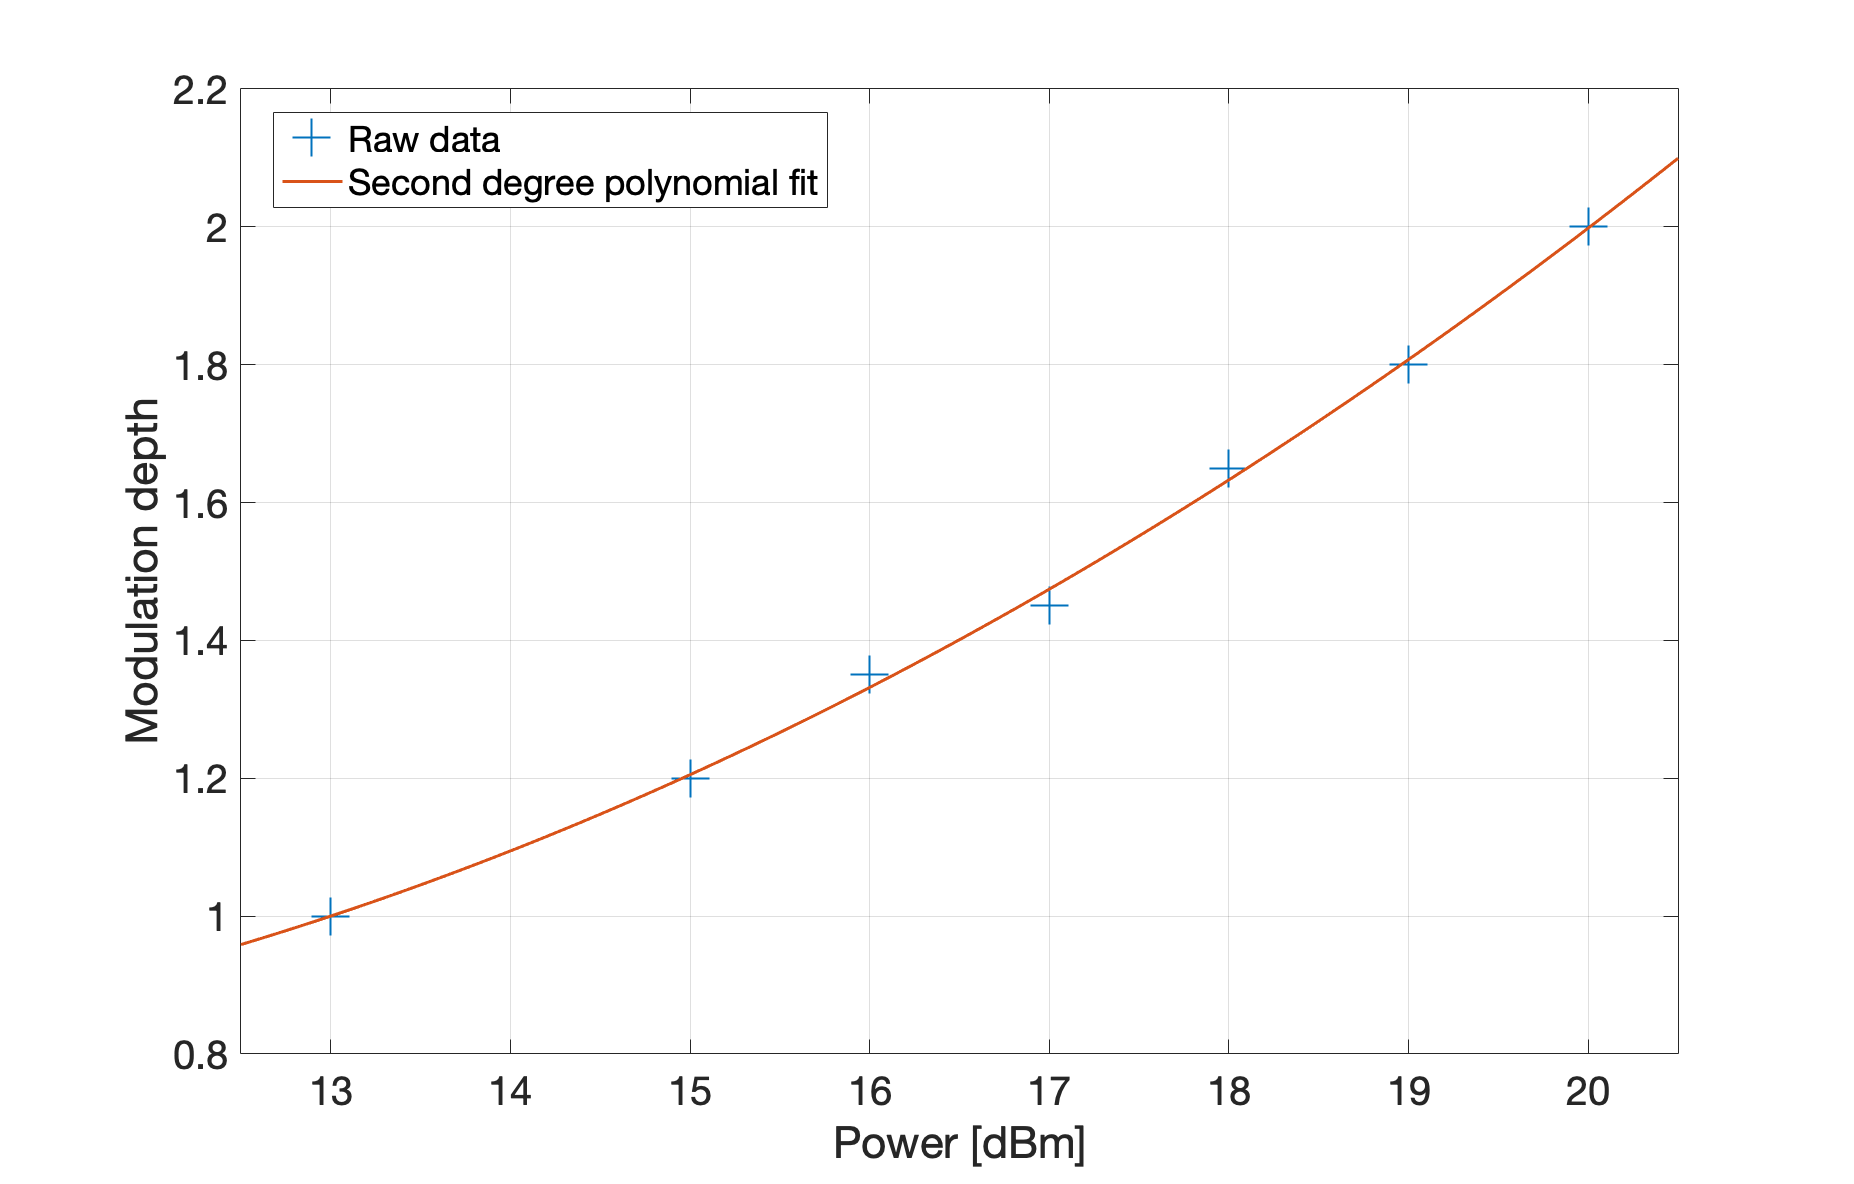
\includegraphics[width=.7\textwidth]{exp-tf-reservoir/mod_depth.png}
	\caption{Modulation depth $m$ as a function of the modulation power [dBm] and second degree polynomial interpolation for $\pulsefreq{\omegamod}=\SI{19.9943}{\giga\hertz}$}
	\label{mod_depth}
\end{figure}

On figure \ref{mod_depth}, one can see the data, as well as the second degree polynomial interpolation. The experimental points only start at 13 dBm because below this value, the side peak was too small to lead significant measures. As already claimed, one cannot go above $m = 2$ experimentally because the RF generator is not able to supply modulation powers higher than 20 dBm at such high modulation frequencies. The empirical polynomial relation is:

\begin{equation}
	m(P[\textrm{dBm}]) = \num{8.004d-3} P^2[\textrm{dBm}] - 0.1215 P[\textrm{dBm}] + 1.222
\end{equation}

It was decided not to go further that a second degree polynomial interpolation because the results were already satisfying.

%%%%%%%%%% PDH STABILISATION TECHNIQUE %%%%%%%%%%

\section{Pound-Drever-Hall stabilisation technique}

\label{sec-pdh}

In this section, the \gls{pdh} stabilisation technique is presented. First, the rationale behind its introduction is discussed. After that, it is shown that the error function resulting from the \gls{pdh} modulation reveals new informations about the phase of the electric field inside the cavity that allow to reach better stabilisation performances.

%%% INTRODUCTION %%%

\subsection{Introduction}

The \gls{pdh} stabilisation technique was proposed in 1983 in \cite{drever1983laser} and since then has proven to be a powerful scheme enabling to accurately stabilise optical cavities. Among other applications, it has been used to to stabilise the laser and measure the thermal noise in the arms of the Michelson interferometer of the LIGO \cite{black1998notes}, which made possible the observation of gravitational waves.\\

The basic idea of the \gls{pdh} technique is to modify the transfer function of the cavity in such a way that its observation will provide more information about the phase. This is implemented in practice by using an additional \gls{pm} and some electronic post-processing, which is handled by the Digilock in our setup.

\subsubsection{Cavity stabilisation}

Before discussing the \gls{pdh} scheme, the principles of cavity stabilisation are presented. As a reminder, this action consists in keeping the relative phase between the electric field inside the cavity after a round trip and the incident electric field equal to a given reference value. Its value can be estimated by measuring the power reflected by the cavity, and can be modified by using actuators to change either the length of the cavity, or the emission wavelength of the laser. \\

\begin{figure}
	\centering
	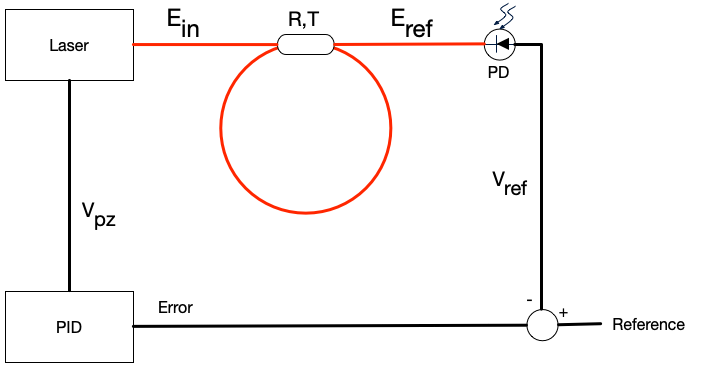
\includegraphics[width=.7\textwidth]{cavity_stab_principle}
	\caption{Schematic representation of cavity stabilisation}
	\label{cavity_stab_principle}
\end{figure}

On figure \ref{cavity_stab_principle}, one can observe the basic principle of the regulation of an optical cavity. The top branch of the figure is well-known at this point. The incident field $E_{\text{in}}$ enters the cavity at the level of the coupler, where the reflected $E_{\text{ref}}$ exits the cavity. The latter is then measured by the \gls{pd}. Henceforth, the different elements should be looked at under the light of control theory. The measured tension $V_{\text{ref}}$ is compared to a reference, which is the value that the regulator is trying to maintain. The difference between the reference and the measured tension is the error, which is processed by a device called the \gls{pid} regulator. In all generality, a \gls{pid} regulator, or \gls{pid} in short, is governed by this equation in the time domain \cite[p.196]{franklin2015feedback}:

\begin{equation}
	u(t) = k_P e(t) + k_I \int_{-\infty}^t e(\tau) d\tau + k_D \frac{de}{dt}(t)
\end{equation}

With $u(t)$ the output of the \gls{pid}, which is in this context the tension applied to the piezoelectric $V_{\text{pz}}$, $e(t)$ the error and $k_I$, $k_P$ and $k_D$ the proportional, integral, and differential coefficients, respectively. In order to get the \gls{pid} to work, one needs to tune those three coefficients, either using analytical methods, or heuristically by scanning the different values. The latter option was the one followed in the experimental implementations described in this work.\\

The voltage $V_{\text{pz}}$, the output of the \gls{pid}, is applied to the piezoelectric crystal of the laser and alters its emission wavelength to stay synchronised with the reference.\\

The main limitation of this scheme is linked to the symmetry of the transfer function $\mathcal{R}$. Let us illustrate why the symmetry is a shortcoming by considering a specific situation, with the help of the figure \ref{tf_near_resonance}.  Let us assume an initial condition when one has a cavity stabilised at the resonance, namely at the minimum of the curve. If the cavity is disturbed by any kind of perturbations, the reflected signal will increase, but due to the symmetry with respect to the resonance frequency, how will one know if the phase is increasing or decreasing ? The measured signal will be exactly the same in both situations. This is problematic because instead of rejecting the perturbations, the \gls{pid} could amplify them by interpreting the measured signal in the wrong way. A trick to still be able to stabilise a cavity using this method is to consider not only the instantaneous value of the reflected signal, but also its slope. Doing so, one is able to differentiate between a larger (positive slope) or smaller (negative slope) frequency. Yet, this hack is not recommended because it is more convenient to work only with instantaneous signals. The \gls{pdh} technique overcomes this limitation by introducing a transfer function, called the error function, which is anti-symmetric with respect to the resonance frequencies.

\begin{figure}
	\centering
	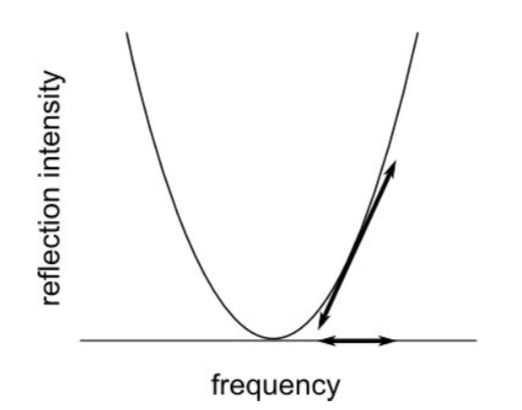
\includegraphics[width=.5\textwidth]{tf_near_resonance}
	\caption{Schematic graph of the transfer function $\mathcal{R}$ near a resonance as function of the frequency \cite{nickersonreview}}
	\label{tf_near_resonance}
\end{figure}

%%% PDH SCHEME %%%

\subsection{Pound-Drever-Hall scheme}

% MATHEMATICAL MODEL %

\subsubsection{Mathematical model}
% Clarify nomenclature

% EXPERIMENTAL RESULTS %

\subsubsection{Experimental results}

%%%%%%%%%% CHARACTERISATION OF THE STABILISATION PERFORMANCE FOR DIFFERENT REGIMES %%%%%%%%%%

\section{Characterisation of the stabilisation performance for different regimes}

%%% APPROACH %%%

\subsection{Approach}

%%% RESULTS %%%

\subsection{Results}